\subsection{Event Builder}
\label{sec:eb}

The Event Builder is the last service in the reconstruction algorithm, and performs a series of functions:

\begin{itemize}
    \item collects information from the upstream services;
    \item correlates information from the sub-detectors into particles;
    \item performs a general particle identification scheme;
    \item organizes the resulting information into a standardized, persistent data bank structure.
\end{itemize}

The service is run twice with identical algorithms, once using hit-based tracks, and later with time-based tracks,
where the results of the hit-based Event Builder are used to initialize time-based tracking.

\subsubsection{Forming Particles}

In defining a reconstructed charged particle in CLAS12, the Event Builder assumes that an assignment will be
made for each reconstructed track in both the Forward Detector and the Central Detector. The associated
calorimeter, scintillator, and Cherenkov detector responses are then assigned to that particle based on
geometric coincidences between the detector responses and the track, with matching criteria corresponding
to the resolution of a given detector. The geometric matching is based on the distance of closest approach
between the track and the response, where an example is shown in Fig.~\ref{fig:ebmatch}.

A similar procedure is followed for creating neutral particles, except the seeding is presently with
unassociated ECAL (for the Forward Detector) and CND (for the Central Detector) responses instead of tracks.

\begin{figure}
\centering
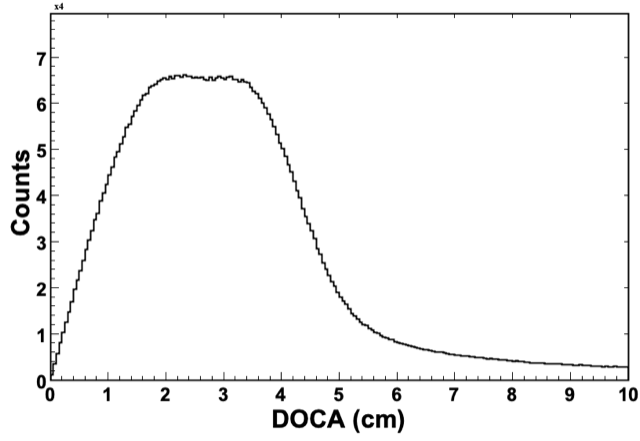
\includegraphics[width=0.45\textwidth,height=0.2\textheight]{pics/pcal-doca.png}
\caption{Example of the geometric matching criteria showing the distance of closest approach between a charged
  track from the DC extrapolated to the ECAL and the cluster positions in the ECAL.}
  \label{fig:ebmatch}
\end{figure}

\subsubsection{Event Start Time}

A start time is assigned to the entire event and serves as our most precise reference time on which all time-based
particle identification relies. This is based on the optimal charged particle candidate in the Forward Detector with
an associated FTOF timing response. The Event Builder assigns the start time based on the highest energy electron
in the ECAL. If there is no electron in the ECAL, it next looks for a positron in the ECAL. If there is no lepton, the
next track in the priority list is a forward-going positive track (assumed to be a $\pi^+$). Finally, if there is no
forward-going positive track, it looks for a forward-going negative track (assumed to be a $\pi^-$). When looking
for $\pi^+$ or $\pi^-$ tracks, only the candidate with the highest momentum in each group is considered.

A parallel event start time is determined from the FT to facilitate physics analyses and triggers where the
primary scattered electron is at very forward angles in the FT. In this case, all combinations of charged particles
in the FT and the Forward Detector are considered. The particle in the FT is assumed to be an electron, whereas
all hadron mass hypotheses are considered for the Forward Detector tracks. The combination with the best time
coincidence is chosen. The timing of the resulting FT electron is then used to assign the start time.

A correction to the start time is then performed using the RF signal from the accelerator, combined with the
reconstructed event vertex position. This effectively aligns the event start time to our best measure of the
beam-bunch arrival time at the target.

The uncorrected, measured vertex time of a particle, $t_v$, can be written as
\begin{equation}
    t_v = t-\frac{P_L}{\beta c},
\end{equation}

\noindent
where $t$ is the measured time response (e.g. in a scintillator), $P_L$ is the path length between the primary
interaction vertex and that response, and $\beta c$ is the speed of the particle.  We can then construct a
correction to align this time with the closest beam bunch time at the target:

\begin{eqnarray}
\Delta t_{RF}\!\!\!\!&=&\!\!\!\! t_v + (z_0-z_v)/c - t_{RF} - N/(2 f_{RF}),\\
\Delta t'_{RF}\!\!\!\!&=&\!\!\!\! mod(\Delta t_{RF},1/f^{RF})-1/(2 f_{RF}),  \nonumber
\end{eqnarray}

\noindent
where $f_{RF}$ is the frequency of the accelerator, 249.5~MHz or 499~MHz, corresponding to 2.004~ns or
4.008~ns bunch spacings, $t_{RF}$ is the measured, calibrated RF time for the event, and $z_0$ is the target
center and enters due to its use as a position calibration reference. The resulting RF- and vertex-corrected
start time for the event is then given as

\begin{equation}
  \label{eq:starttime}
t'_v = t_v - \Delta t'_{RF}.
\end{equation}

\subsubsection{Particle Identification}

The next stage is a basic particle identification scheme.  This is intended to be loose to accommodate a variety of
physics analyses, while persisting the necessary information to easily tighten and improve the criteria later.

For charged particles, first calorimetry and Cherenkov information is used to positively identify $e^-/e^+$
candidates in the Forward Detector. If the measured energy deposition is consistent with the expected sampling
fraction of the ECAL, and the photoelectron response from the HTCC is consistent with $\beta\sim1$, the particle
is assigned as an $e^-$ or $e^+$ depending on sign of the curvature of the track from forward tracking with the
DCs through the torus magnetic field. 

The remaining charged particles are then assumed to be hadrons and assigned an identity based solely on timing
information, where the $p/K/\pi$ candidate giving the smallest time residual is assigned. This time residual is
computed from the difference between the measured particle flight time and that computed for a given mass
hypothesis. Figure~\ref{fig:betavsp} shows reconstructed $\beta$ vs. momentum distributions from beam data
for forward-going positively charged hadrons using information from the FTOF and DC subsystems, where the
electron is reconstructed either in the Forward Detector (Fig.~\ref{fig:betavsp}(top)) or in the Forward Tagger
(Fig.~\ref{fig:betavsp}(bottom)). The computed curves for the different mass hypotheses are overlaid.

\begin{figure}[t]
\centering
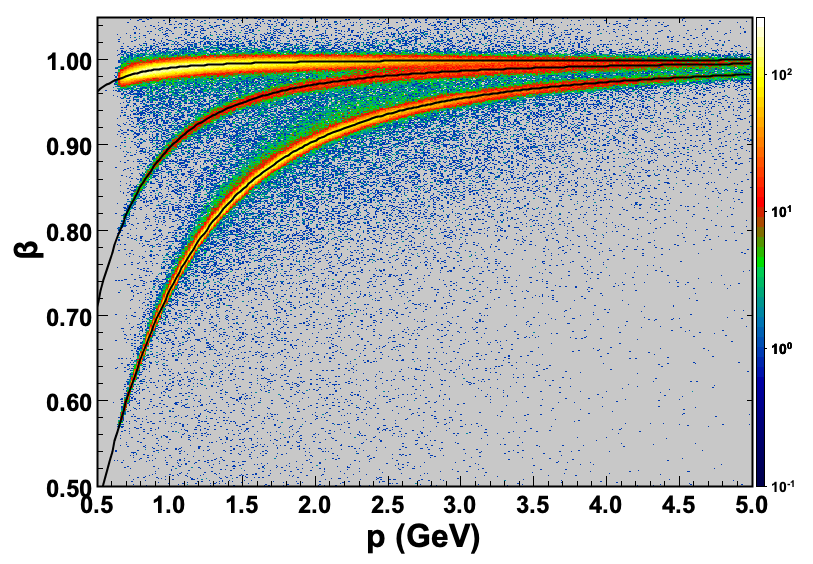
\includegraphics[width=0.45\textwidth]{pics/ftof_betap.png}
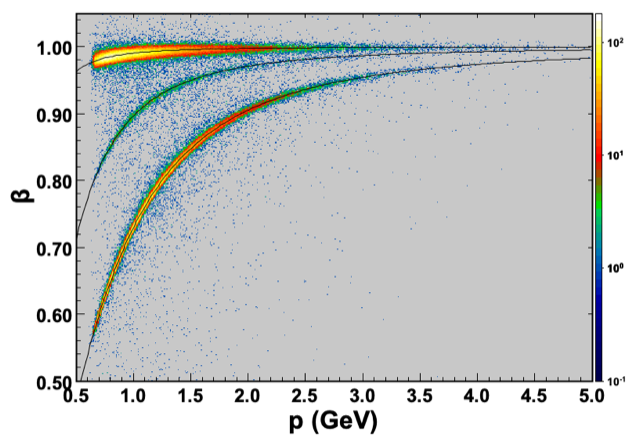
\includegraphics[width=0.45\textwidth]{pics/ft_betap.png}
\caption{Particle $\beta$ vs. momentum from simulation data for positively charged tracks with their start time
  from an electron in the Forward Detector (top plot) or in the FT (bottom plot).}
\label{fig:betavsp}
\end{figure}

Identification of neutral particles assumes only neutrons and photons, differentiated only by timing and
topological information. For the Forward Detectors this is based on the ECAL, while for the Central Detector it
is based on the CND, and their reconstructed cluster positions are used to compute the particle travel path from
the event vertex, assuming a straight-line trajectory. If the resulting measured $\beta$ is close to 1, the particle
is assigned as a photon, otherwise it is assigned as a neutron. For photons in the Forward Detector, the momentum
is determined from its deposited energy and ECAL sampling fraction~\cite{ecal-nim}. For neutrons, the momentum
is assigned based on the measured $\beta$, assuming the neutron mass. Figure~\ref{fig:neutbeta} shows an
example of $\beta$ reconstructed for neutrals in the Forward Detector showing separation of photons and neutrons.

\begin{figure}
\centering
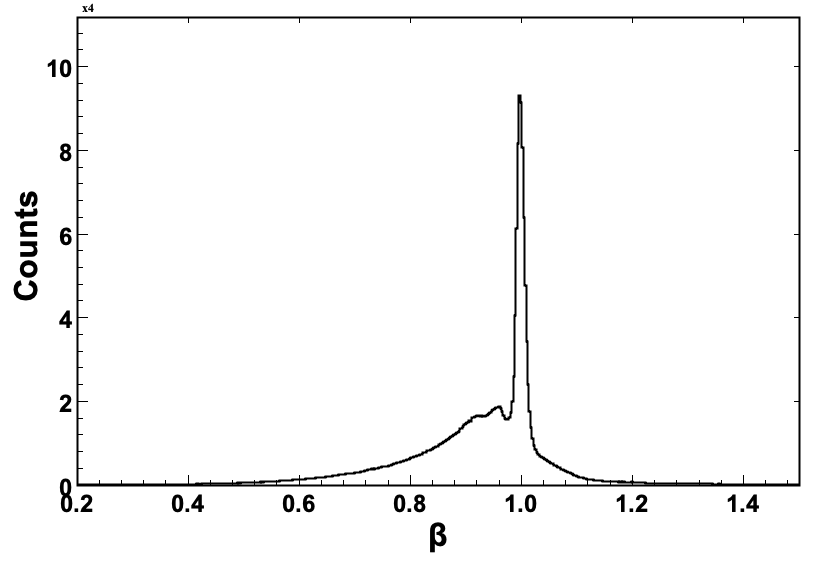
\includegraphics[width=0.45\textwidth]{pics/neutral_beta.png}
\caption{$\beta$ distribution for neutral particles as measured by the ECAL from simulation data, showing a sharp
  peak at $\beta=1$ from photons and a broader, slower distribution from neutrons.}
\label{fig:neutbeta}
\end{figure}

A particle identification quality factor in the form of a signed-$\chi$, or pull, is assigned based on the individual
contributing detector subsystem responses and their resolutions. For $e^-/e^+$ identification the
resolution-normalized distance from the expected ECAL sampling fraction is used, while for charged hadrons the
resolution normalized time-difference is used. The resulting information is organized into standardized output
bank structures for physics analysis, see Section~\ref{sec:dsts}. This includes the particle four-vectors, the
associated detector responses, and global event information such as beam RF and helicity information.

\subsubsection{Particle Identification Performance}

The accuracy of the particle identification algorithm that is currently implemented can be estimated from
Monte Carlo simulations where the assigned particle identification can be compared to the true one.
Tables~\ref{table:pidmatrix} and~\ref{table:pidmatrix2} show the particle identification matrix for the Forward
and Central Detectors, respectively. The values are based on simulations of electron-hadron or electron-photon
pairs with hadron and photon momenta in the range from 1 to 2.5~GeV and electron momenta in the range from 1 to
9~GeV. The diagonal elements correspond to the cases where the particle is correctly identified and the off-diagonal
elements to the cases where the particle is misidentified. It should be noted that the resulting values are strictly
related to the assignment algorithm currently in use and on the timing resolutions implemented in the Monte Carlo
simulation~\cite{sim-nim}. An increase of the diagonal element values and a corresponding decrease of the
misidentification probability is expected as, for example, information from the threshold Cherenkov detectors and
the RICH in particular are integrated into the algorithm and isolated hits in the FTOF and CTOF detectors are
incorporated into the neutral particle identification algorithm.

\begin{table}[ht]
  \begin{center}
    \begin{tabular}{|c|cccccc|}\hline
          & \multicolumn{6}{c|}{Truth}\\        
          & $e$  & $\pi$ & $K$  & $p$  & $n$  & $\gamma$ \\\hline
  $e$     & 0.98 &       &      &      &      &          \\ 
  $\pi$   &      &  0.93 & 0.10 & 0.00 &      &          \\ 
  $K$     &      &  0.03 & 0.80 & 0.00 &      &          \\ 
  $p$     &      &  0.03 & 0.02 & 0.98 &      &          \\ 
  $n$     &      &       &      &      & 0.66 &   0.01   \\ 
 $\gamma$ &      &       &      &      & 0.14 &   0.95   \\\hline 
    \end{tabular}  
    \caption{Particle identification matrix for the CLAS12 Forward Detector based on simulated hadrons and
      photons with momentum between 1 and 2.5~GeV, and electrons up to 9~GeV. The diagonal elements are
      correctly identified, while the off-diagonal elements are misidentified. Detector inefficiencies are included.}
  \label{table:pidmatrix}
  \end{center}
\end{table}

Another measure of the particle identification performance for neutrals is given by the reconstruction of $\pi^0$
decays to two photons. Figure~\ref{fig:pi0mass} shows the $\gamma \gamma$ invariant mass reconstructed from
the ECAL and from the Forward Tagger.

\begin{table}[ht]
  \begin{center}
    \begin{tabular}{|c|cccc|}\hline
          & \multicolumn{4}{c|}{Truth}\\        
          & $\pi$ & $K$  & $p$  & $n$  \\\hline
  $\pi$   &  0.84 & 0.14 & 0.00 &      \\ 
  $K$     &  0.11 & 0.80 & 0.01 &      \\ 
  $p$     &  0.03 & 0.04 & 0.95 &      \\ 
  $n$     &       &      &      & 0.11 \\ 
 $\gamma$ &       &      &      & 0.00 \\\hline 
    \end{tabular}  
    \caption{Particle identification matrix for the CLAS12 Central Detector based on simulated hadrons with momentum
      between 0.3 and 1.1~GeV. The diagonal elements are correctly identified, while the off-diagonal elements
      are misidentified. Detector inefficiencies are included.}
  \label{table:pidmatrix2}
  \end{center}
\end{table}

\begin{figure}[t]
\centering
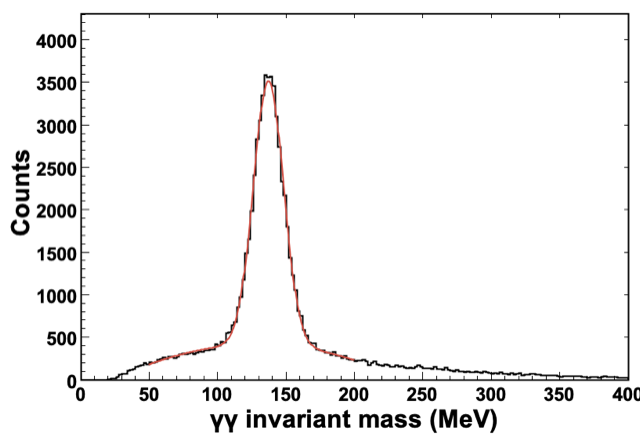
\includegraphics[width=0.45\textwidth]{pics/ecal_pi0.png}
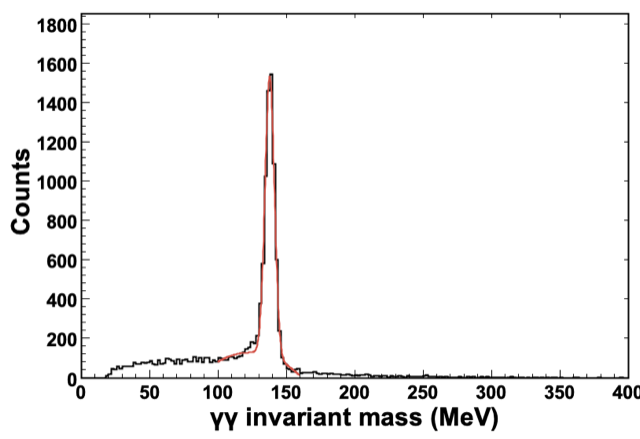
\includegraphics[width=0.45\textwidth]{pics/ft_pi0.png}
\caption{Reconstructed $\pi^0 \to \gamma \gamma$ candidates using photons detected in the ECAL (top plot) and
  the FT (bottom plot). The plots are based on simulations of semi-inclusive deep inelastic scattering events
  generated based on the PYTHIA event generator~\cite{clasdis}.}
\label{fig:pi0mass}
\end{figure}

